\documentclass[aspectratio=169,11pt]{beamer}

\usepackage[T1]{fontenc}
\usepackage[utf8]{inputenc}
\usepackage{lmodern}
\usepackage{amsmath}
\usepackage{booktabs}
\usepackage{graphicx}

% Keep the visual style simple; edit these colors to customize the template.
\usetheme{Madrid}
\definecolor{studyblue}{HTML}{173B57}
\definecolor{studyteal}{HTML}{087F8C}
\setbeamercolor{structure}{fg=studyblue}
\setbeamercolor{alerted text}{fg=studyteal}
\setbeamertemplate{navigation symbols}{}
\setbeamertemplate{footline}[frame number]
\graphicspath{{figures/}{../}}

% TODO: Replace the author, affiliation, and date before presenting.
\title[PINN collocation]{Collocation Dynamics in Physics-Informed Neural Networks}
\subtitle{Adaptive sampling, diffusion, and solution sharpness}
\author{Hiero de Paula, Sofia Suesdek}
\institute{Escola Politécnica da Universidade de São Paulo}
\date{\today}

\begin{document}

\begin{frame}[plain]
  \titlepage
\end{frame}

\section{Collocation dynamics and research questions}

% Introduce the scientific variable without repeating a general PINN tutorial.
\begin{frame}{Why study collocation dynamics?}
  The physics loss is evaluated on a finite set of points:
  \[
    \mathcal{L}_{\mathrm{PDE}}(\theta;Z)
      = \frac{1}{N}\sum_{i=1}^{N}r_\theta(z_i)^2,
      \qquad z_i=(x_i,t_i).
  \]
  \begin{itemize}
    \item Point locations determine where the PDE is enforced during training.
    \item Keeping, replacing, or moving points changes coverage and the
      optimization trajectory, even at the same point budget.
    \item Concentrating points near difficult features may help, while leaving
      other regions insufficiently constrained.
  \end{itemize}
  \begin{block}{What must be evaluated independently?}
    A small residual at training points does not guarantee a small residual
    throughout the domain or an accurate solution.
  \end{block}
\end{frame}

\begin{frame}{Five ways to place the same interior point budget}
  \small
  \begin{tabular}{@{}p{0.27\textwidth}p{0.69\textwidth}@{}}
    \toprule
    Method & Interior point strategy \\
    \midrule
    Fixed Hammersley & Keep the initial low-discrepancy design. \\
    Random resampling & Periodically replace points with fresh uniform random points. \\
    RAD\textsuperscript{\cite{rad}} & Sample fresh candidates preferentially where residual magnitude is large. \\
    PACMANN\textsuperscript{\cite{pacmann}} & Move points along the coordinate gradient of squared residual,
      using Adam ascent. \\
    PACMANN + diffusion & Add domain-scaled Gaussian perturbations to the
      coordinate-Adam motion. \\
    \bottomrule
  \end{tabular}
  \begin{block}{Residual-based selection versus gradient-based adaptive sampling}
    RAD selects a new population using residual scores; PACMANN moves the
    current population using $\nabla_{(x,t)}r_\theta^2$.
  \end{block}
\end{frame}

\begin{frame}{Research questions}
  \begin{enumerate}
    \item How does the benefit of point-adaptive collocation change across
      solution-sharpness regimes, for solution and PDE-residual error?
    \item Does adding diffusion to PACMANN improve either outcome, and does
      the effect depend on the regime?
  \end{enumerate}
  \medskip
  \begin{block}{Working hypothesis}
    Gradient-adaptive methods may offer greater benefits for solutions with
    sharp features. Both the adaptive-sampling and diffusion benefits remain
    open questions.
  \end{block}
  \smallskip
  Sharp solution gradients and coordinate gradients of residual scores are
  different quantities.
\end{frame}

\section{Problem, implementation, and reference validation}

\begin{frame}{Starting problem: viscous Burgers equation}
  \[
    \partial_t u + u\,\partial_x u - \nu\,\partial_{xx}u = 0,
    \qquad (x,t)\in[-1,1]\times[0,0.99].
  \]
  \[
    u(x,0)=-\sin(\pi x), \qquad u(-1,t)=u(1,t)=0.
  \]
  \begin{itemize}
    \item Viscosity $\nu$ controls diffusion in the PDE and the solution regime.
    \item Train from the PDE and fixed initial/boundary constraints.
    \item Use numerical reference solutions only for evaluation.
  \end{itemize}
  \begin{block}{Two distinct parameters}
    $\nu$ changes the physical problem; $\sigma$ controls stochastic diffusion
    of collocation points in PACMANN + diffusion.
  \end{block}
\end{frame}

\begin{frame}{From the released PACMANN code to a controlled study}
  \small
  \begin{tabular}{@{}p{0.15\textwidth}p{0.81\textwidth}@{}}
    \toprule
    Category & Implementation choice \\
    \midrule
    Retained & Four 64-neuron tanh layers, float64, five alternating Adam/L-BFGS
      stages, upstream sampler settings and coordinate-Adam procedure. \\
    Changed & Match 2,500 interior PDE points from initialization for every
      method; keep initial/boundary constraints fixed. Use generated references
      and common final-checkpoint evaluation. \\
    Added / tuned & Gaussian diffusion of point coordinates; select its
      coefficient separately at each viscosity on development seeds. \\
    \bottomrule
  \end{tabular}
  \medskip
  \begin{itemize}
    \item DeepXDE with a PyTorch backend, adapted from the released implementation.
    \item Evaluate final models and retain all planned seeds, including failures.
    \item Record actual optimizer work; shared limits do not imply equal computation.
  \end{itemize}
  {\footnotesize These are disclosed controlled-study choices. Published-result
    reproduction has not been established.}
\end{frame}

\begin{frame}{Reference generation and validation at $\nu=0.01/\pi$}
  \begin{columns}[T,onlytextwidth]
    \begin{column}{0.42\textwidth}
      \small
      \textbf{Generated reference}
      \begin{itemize}
        \item Chebyshev spatial collocation, degree $N=1024$.
        \item Radau time integration.
        \item Compare on the original 256 spatial points and 100 snapshot times.
      \end{itemize}
      \textbf{Two different checks}
      \begin{itemize}
        \item Reference disagreement:\\
          \alert{0.000319\% relative $L^2$}.
        \item N1024 change in fixed-model error scores:\\
          \alert{less than 0.006\% relative}.
      \end{itemize}
    \end{column}
    \begin{column}{0.55\textwidth}
      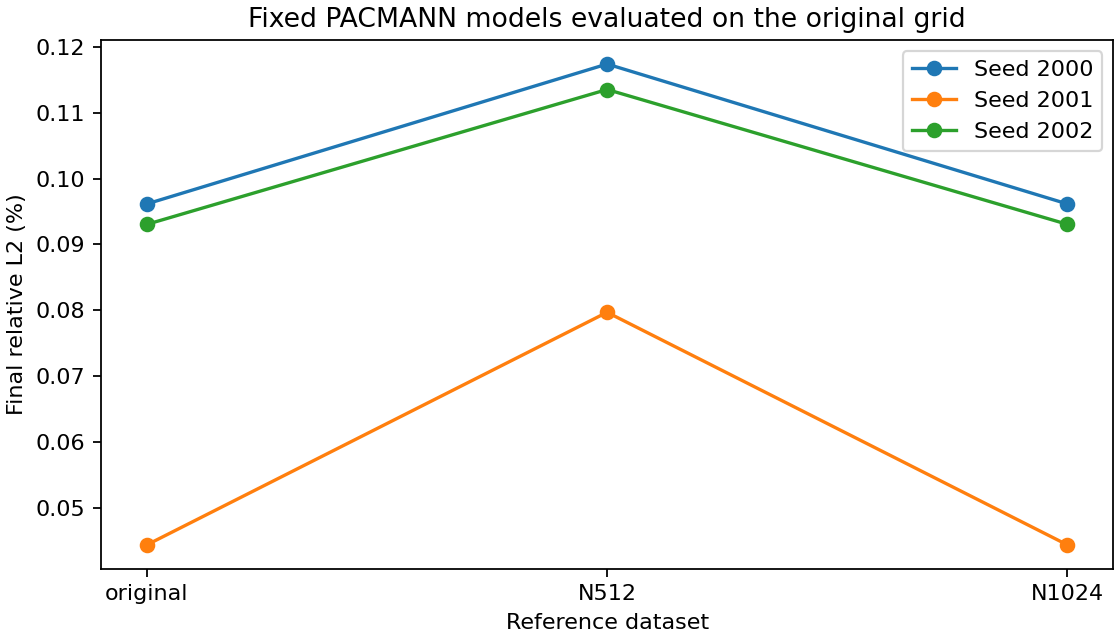
\includegraphics[width=\linewidth]{reference_model_comparison.png}
      \par\smallskip
      {\footnotesize Each line is one fixed trained model. Only the reference
        used to score its predictions changes; no retraining occurs.}
    \end{column}
  \end{columns}
  \medskip
  {\footnotesize Generated values are barycentrically interpolated in space at
    exact shared times. Agreement supports N1024 at this viscosity; it does not
    certify other viscosities or reproduce published training results.}
  % Figure copied unchanged from dataset-validation, commit 035deb16e574d21591b04f9a8fb290ff0e0f1d7e.
  % Source: output/burgers_reference_validation/pacmann_3seed/comparison.png.
\end{frame}

\section{Experimental procedure}

\begin{frame}{Matched training and independent evaluation}
  \begin{columns}[T,onlytextwidth]
    \begin{column}{0.55\textwidth}
      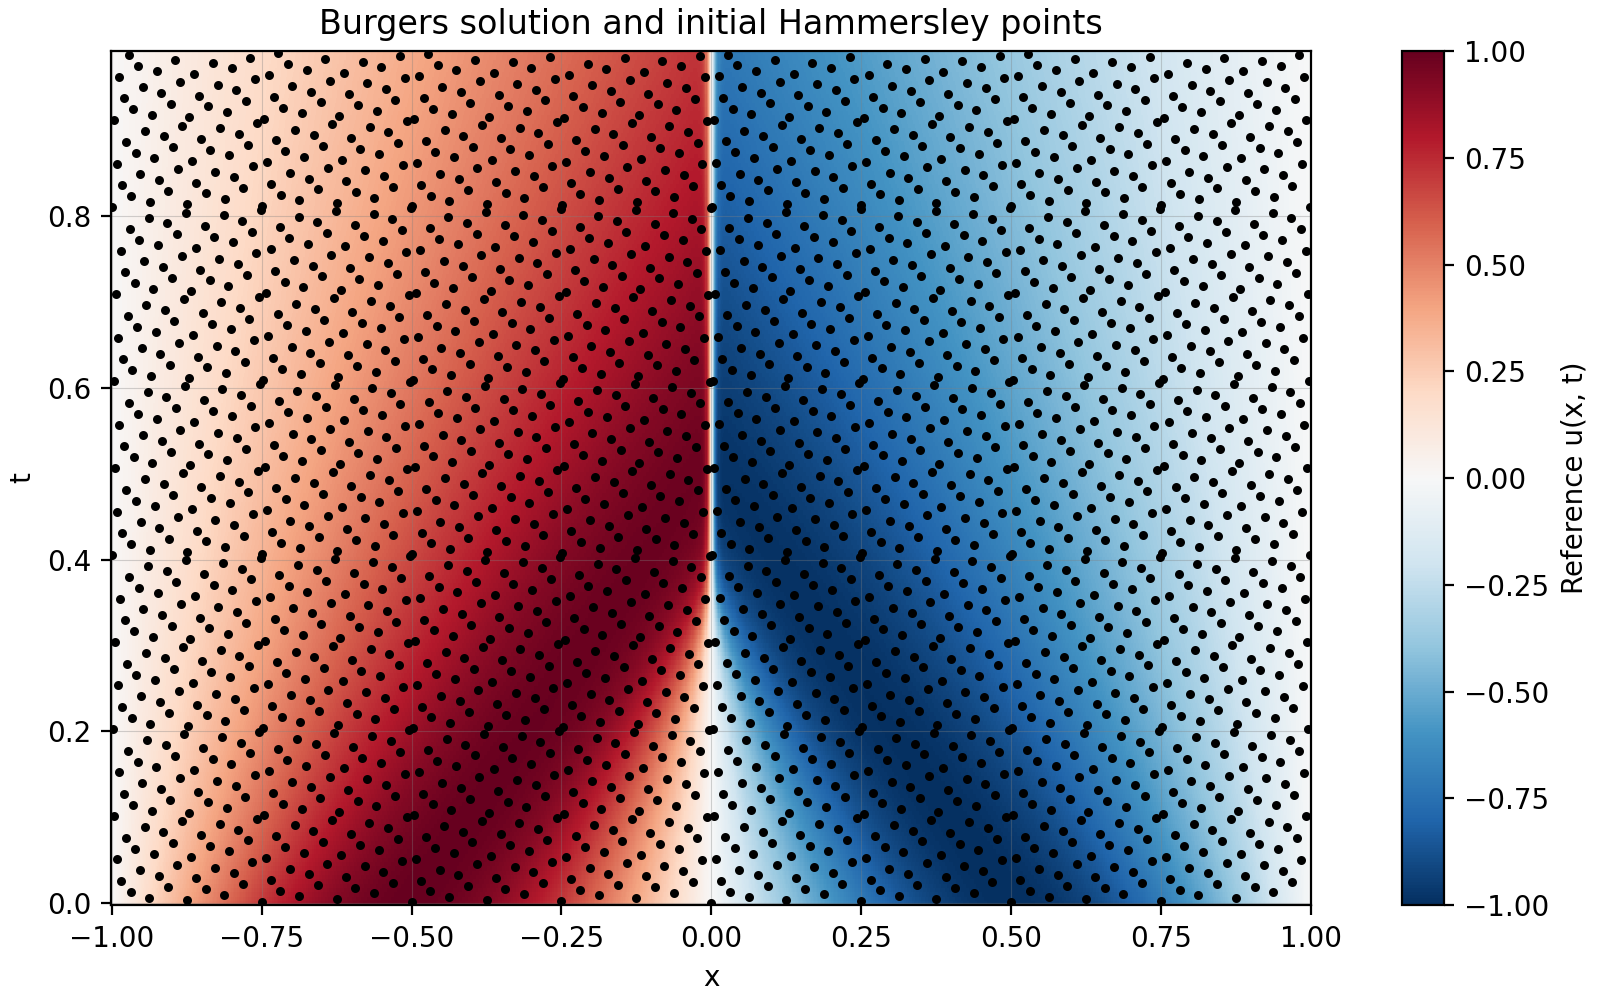
\includegraphics[width=\linewidth]{burgers_initial_collocation.png}
      \par\smallskip
      {\footnotesize Initial Hammersley points at $\nu=0.01/\pi$;
        paired across methods.}
    \end{column}
    \begin{column}{0.42\textwidth}
      \small
      \textbf{Training controls}
      \begin{itemize}
        \item Paired seeds and initial weights.
        \item 2,500 PDE; 80 BC; 160 IC.
        \item Interior updates during Adam only.
      \end{itemize}
      \textbf{Final-model evaluation}
      \begin{itemize}
        \item Solution: uniform $1024\times199$ grid.
        \item Residual RMS: independent $1024\times200$ midpoint grid.
        \item Boundary / initial RMSE.
      \end{itemize}
    \end{column}
  \end{columns}
  \smallskip
  {\footnotesize Float64; DeepXDE 1.14.0 / PyTorch 2.7.1; RTX 5070 (12 GB).
    Ten concurrent seeds per method; method batches run sequentially.}
\end{frame}

\begin{frame}{Tune first, freeze settings, then evaluate}
  \begin{columns}[T,onlytextwidth]
    \begin{column}{0.48\textwidth}
      \begin{block}{Development: three paired seeds}
        \begin{itemize}
          \item Seeds 3000--3002.
          \item Test $\sigma=0$ and positive values $10^{-5},10^{-4},10^{-3},10^{-2}$.
          \item Select by mean final solution relative $L^2$ error.
        \end{itemize}
      \end{block}
    \end{column}
    \begin{column}{0.48\textwidth}
      \begin{block}{Evaluation: ten paired seeds}
        \begin{itemize}
          \item Freeze sigma before using seeds 4000--4009.
          \item Use the same sigma for residual-error evaluation.
          \item Compare all five methods; retain every planned seed.
        \end{itemize}
      \end{block}
    \end{column}
  \end{columns}
  \medskip
  \centering
  Frozen diffusion settings:
  $\nu=0.01/\pi \Rightarrow \sigma=10^{-4}$;\quad
  $\nu=0.01 \Rightarrow \sigma=10^{-3}$.
  \par\medskip
  \raggedright
  {\footnotesize At $\nu=0.01$, zero is a comparison baseline only: select the best
    positive sigma and expand a boundary winner under the approved stopping rule.
    The earlier sweep allowed zero as a candidate. Other samplers retain upstream
    settings; disclose this tuning asymmetry.}
\end{frame}

\section{Results and analysis: reserved for verified campaigns}

% Populate these three frames together after the ongoing nu=0.01 campaign is verified.
\begin{frame}{Results: solution and residual accuracy}
  \begin{block}{Results to be added}
    Complete this comparison after the $\nu=0.01$ campaign is finished and verified.
    Include the accepted $\nu=0.01/\pi$ campaign and the new campaign.
  \end{block}
  \begin{itemize}
    \item TODO: Compare all five methods for both error metrics at each viscosity.
    \item TODO: Show ten-seed means and sample standard deviations; label units.
    \item TODO: Link each table or figure to its frozen campaign and configuration.
  \end{itemize}
  % Accepted numerical evidence: ../results.md and the verified campaign artifacts.
  % Do not insert partial-run rankings or compare tuning errors as held-out results.
\end{frame}

\begin{frame}{Results: variability and paired comparisons}
  \begin{block}{Analysis to be added}
    Use the complete seed sets, including unfavorable and failed outcomes.
  \end{block}
  \begin{itemize}
    \item TODO: Show individual-seed distributions alongside aggregate results.
    \item TODO: Assess paired diffusion-minus-PACMANN changes for both metrics.
    \item TODO: Compare adaptive methods with fixed Hammersley and random resampling.
    \item TODO: Describe large-error outcomes and the sensitivity of means;
      keep any trimmed means supplementary.
  \end{itemize}
  % Retain planned seeds; do not select model-history minima or favorable retries.
\end{frame}

\begin{frame}{Analysis: what changes across viscosities?}
  \begin{block}{Interpretation to be added}
    Connect verified campaign comparisons to the two research questions.
  \end{block}
  \begin{itemize}
    \item TODO: Assess whether the effect of diffusion changes across viscosities.
    \item TODO: Compare method benefits for solution and residual error separately.
    \item TODO: Discuss variability, reference accuracy, and per-viscosity tuning.
  \end{itemize}
  \medskip
  \alert{A viscosity-dependent ranking alone does not establish a sharpness effect.}
  Sharpness and feature-region definitions must be independent of adaptive sampling.
  % Do not infer a mechanism from outcome rankings or partial nu=0.01 results.
\end{frame}

\section{Conclusions}

\begin{frame}{Conclusions, limitations, and next steps}
  \begin{itemize}
    \item \textbf{Evidence:} TODO: State what the completed comparisons support
      about adaptive collocation and diffusion.
    \item \textbf{Limitations:} TODO: Summarize reference accuracy, seed variability,
      and the scope of the tested viscosities.
    \item \textbf{Next step:} TODO: State the next bounded study decision.
  \end{itemize}
  \medskip
  \begin{block}{Interpretation boundary}
    Distinguish observations from hypotheses about their causes. Improvement in
    solution error need not imply improvement in independent residual error.
  \end{block}
\end{frame}

\section{References}
\begin{frame}{References}
  \setbeamertemplate{bibliography item}[text]
  \begin{thebibliography}{2}
    \bibitem{rad}
      C. Wu, M. Zhu, Q. Tan, Y. Kartha, and L. Lu.
      \newblock A comprehensive study of non-adaptive and residual-based adaptive
        sampling for physics-informed neural networks.
      \newblock 2023.
      % Bibliographic metadata verified against github.com/lu-group/pinn-sampling.
    \bibitem{pacmann}
      C. Visser, A. Heinlein, and B. Giovanardi.
      \newblock PACMANN: Point adaptive collocation method for artificial neural networks.
      \newblock 2025.
  \end{thebibliography}
  \medskip
  \small
  Released-code provenance and controlled-study deviations are recorded in
  \texttt{references/upstream.md}.
  % TODO: Add a primary PINN reference if its derivation is presented.
\end{frame}

% Backup slides support questions and are excluded from the main-slide counter.
\section*{Backup}
\setbeamertemplate{footline}{}

\begin{frame}[noframenumbering]{Backup: detailed scientific settings}
  \footnotesize
  \begin{tabular}{@{}p{0.25\textwidth}p{0.71\textwidth}@{}}
    \toprule
    Setting & Frozen configuration \\
    \midrule
    Network / precision & $2$--$64$--$64$--$64$--$64$--$1$, tanh, Glorot normal;
      float64. \\
    Point budgets & 2,500 interior PDE points; 80 boundary and 160 initial points. \\
    Optimizer schedule & Five phases, each with 7,000 Adam steps at $10^{-3}$,
      followed by L-BFGS. \\
    L-BFGS limits & Nominal maxiter 3,000, maxfun 3,750; maxcor 100,
      gtol $10^{-8}$, ftol 0. \\
    Sampling cadence & Every 50 Adam steps; no point updates during L-BFGS. \\
    PACMANN motion & 15 coordinate steps at $10^{-5}$;
      $\beta_1=0.9$, $\beta_2=0.999$, $\epsilon=10^{-7}$ outside the square root. \\
    RAD & 100,000 candidates; weight $|r|/\operatorname{mean}(|r|)+1$;
      sample without replacement. \\
    Diffusion convention & Per coordinate step, add independent Gaussian noise
      with componentwise standard deviation $\sigma (L_x,L_t)/\sqrt{15}$. \\
    Evaluation & Uniform solution grid $1024\times199$ with spatial barycentric
      reference interpolation; independent residual grid $1024\times200$. \\
    \bottomrule
  \end{tabular}
  \par\medskip
  The retained DeepXDE L-BFGS driver can exceed nominal stage limits.
  Report recorded iterations, function evaluations, and training time.
  % Source: the two frozen campaign YAMLs and references/upstream.md.
\end{frame}



\end{document}
